% The following \documentclass options may be useful:
%
% preprint      Remove this option only once the paper is in final form.
% 10pt          To set in 10-point type instead of 9-point.
% 11pt          To set in 11-point type instead of 9-point.
% authoryear    To obtain author/year citation style instead of numeric.
\documentclass[preprint,nonatbib,10pt,nocopyrightspace]{sigplanconf}

%%%%%%%%%%%%%%%%%%%%%%%%%
%% Document and Layout %%
%%%%%%%%%%%%%%%%%%%%%%%%%

% Fix for multiple "No room for a new \dimen" errors.
%
% See: http://tex.stackexchange.com/questions/38607/no-room-for-a-new-dimen
%
\usepackage{etex}

\usepackage[utf8]{inputenc}

% Fix for "'babel/polyglossia' detected but 'csquotes' missing"
% warning. NOTE: Include after inputenc.
%
\usepackage{csquotes}

\usepackage{booktabs}

% Required for full page-width tables.
\usepackage{tabularx}

% Define column types L, C, R with known text justification and fixed
% widths:
\usepackage{array}
\newcolumntype{L}[1]{>{\raggedright\let\newline\\\arraybackslash\hspace{0pt}}m{#1}}
\newcolumntype{C}[1]{>{\centering\let\newline\\\arraybackslash\hspace{0pt}}m{#1}}
\newcolumntype{R}[1]{>{\raggedleft\let\newline\\\arraybackslash\hspace{0pt}}m{#1}}

% Make internal macro definitions accessible,
% e.g. \@title, \@date \@author.
\makeatletter

% Uncomment the following line to remove column separation:
%
%\setlength{\columnsep}{5mm}

\usepackage{color}
\newcommand{\fix}[1]{\textcolor{red}{\em\footnotesize#1}}


%%%%%%%%%%%%%%%%
% Bibliography %
%%%%%%%%%%%%%%%%
\usepackage[%
    backend=biber,%bibtex,
    style=numeric-comp,
    % style=numeric-comp,  % numerical-compressed
    sorting=none,        % nty,nyt,nyvt,anyt,anyvt,ynt,ydnt,none
    sortcites=true,      % sort \cite{b a d c}: true,false
    block=none,          % space between blocks: none,space,par,nbpar,ragged
    indexing=false,      % indexing options: true,false,cite,bib
    citereset=none,      % don't reset cites
    isbn=false,          % print ISBN?
    url=true,            % print URL?
    doi=false,           % print DOI?
    natbib=true,         % natbib compatability
    maxbibnames=99       % no 'et-al' in the bibliography pls
  ]{biblatex}

\addbibresource{../../../library.bib}

% Reduce the font size of the bibliography:
\renewcommand{\bibfont}{\normalfont\scriptsize}


%%%%%%%%%%%%%%%%%%%%%%%%%%%%%%%%%%%%%
%% Figures, footnotes and listings %%
%%%%%%%%%%%%%%%%%%%%%%%%%%%%%%%%%%%%%

\usepackage[perpage]{footmisc}

% Pre-requisites for rendering upquotes in listings package.
\usepackage[T1]{fontenc}
\usepackage{lmodern}
\usepackage{textcomp}

% Source code listings.
\usepackage{listings}
\lstset{%
  basicstyle=\scriptsize,%
  breaklines=true,%
  postbreak=\raisebox{0ex}[0ex][0ex]{\ensuremath{\color{red}\hookrightarrow\space}},% red arrow at line breaks
  captionpos=b%
}

% OpenCL listings
%
% From: http://gpumodeling.blogspot.com/2011/06/opencl-programs-in-latex-listings.html
 \lstdefinelanguage[OpenCL]{C}[ANSI]{C}
{morekeywords={__kernel,kernel,__local,local,__global,global,%
__constant,constant,__private,private,%
char2,char3,char4,char8,char16,%
uchar2,uchar3,uchar4,uchar8,uchar16,%
short2,short3,short4,short8,short16,%
ushort2,ushort3,ushort4,ushort8,ushort16,%
int2,int3,int4,int8,int16,%
uint2,uint3,uint4,uint8,uint16,%
long2,long3,long4,long8,long16,%
ulong2,ulong3,ulong4,ulong8,ulong16,%
float2,float3,float4,float8,float16,%
image2d_t,image3d_t,sampler_t,event_t,%
bool2,bool3,bool4,bool8,bool16,%
half2,half3,half4,half8,half16,%
quad,quad2,quad3,quad4,quad8,quad16,%
complex,imaginary},%
}%

% Pseudo-code listings.
\usepackage{algorithm}
\usepackage{algpseudocode}
\newcommand{\Break}{\State \textbf{break} }
\algblockdefx[Loop]{Loop}{EndLoop}[1][]{\textbf{Loop} #1}{\textbf{End
    Loop}}

\algrenewcommand\ALG@beginalgorithmic{\footnotesize}


%%%%%%%%%%%%%%%%%%%%%%%%
%% Graphics and maths %%
%%%%%%%%%%%%%%%%%%%%%%%%
\usepackage{amsmath}
\usepackage{tikz}

% Tikz flowchart configuration.
\usetikzlibrary{shapes,arrows,shadows,fit,backgrounds}
\tikzstyle{decision} = [diamond,
                        draw,
                        text width=4.5em,
                        text badly centered,
                        node distance=3cm,
                        inner sep=0pt]
\tikzstyle{block}    = [rectangle,
                        draw,
                        text width=5em,
                        text centered,
                        node distance=3cm,
                        minimum height=4em,
                        inner sep=.2cm]
\tikzstyle{line}     = [draw, -latex']

% Vector notation, e.g. \vv{x}:
%
\usepackage{esvect}

% Additional amsmath symbols, see:
%
% http://texblog.org/2007/08/27/number-sets-prime-natural-integer-rational-real-and-complex-in-latex/
%
\usepackage{amsfonts}
\usepackage{amssymb}

\usepackage{graphicx}
\usepackage{mathtools}

% Provide bold font face in maths.
\usepackage{bm}

\usepackage{subcaption}
\expandafter\def\csname ver@subfig.sty\endcsname{}

% Define an 'myalignat' command which behave as 'alignat' without the
% vertical top and bottom padding. See:
%     http://www.latex-community.org/forum/viewtopic.php?f=5&t=1890
\newenvironment{myalignat}[1]{%
  \setlength{\abovedisplayskip}{-.7\baselineskip}%
  \setlength{\abovedisplayshortskip}{\abovedisplayskip}%
  \start@align\z@\st@rredtrue#1
}%
{\endalign}

% Define additional operators:
\DeclareMathOperator*{\argmin}{arg\,min}
\DeclareMathOperator*{\argmax}{arg\,max}

\DeclareMathOperator*{\gain}{Gain}

% Skeleton operators.
\DeclareMathOperator*{\map}{Map}
\DeclareMathOperator*{\reduce}{Reduce}
\DeclareMathOperator*{\scan}{Scan}
\DeclareMathOperator*{\stencil}{Stencil}
\DeclareMathOperator*{\zip}{Zip}
\DeclareMathOperator*{\allpairs}{All\,Pairs}

% Define a command to allow word breaking.
\newcommand*\wrapletters[1]{\wr@pletters#1\@nil}
\def\wr@pletters#1#2\@nil{#1\allowbreak\if&#2&\else\wr@pletters#2\@nil\fi}

% Define a command to create centred page titles.
\newcommand{\centredtitle}[1]{
  \begin{center}
    \large
    \vspace{0.9cm}
    \textbf{#1}
  \end{center}}

% Provide generic commands \degree, \celsius, \perthousand, \micro
% and \ohm which work both in text and maths mode.
\usepackage{gensymb}

\begin{document}

\special{papersize=8.5in,11in}
\setlength{\pdfpageheight}{\paperheight}
\setlength{\pdfpagewidth}{\paperwidth}

\conferenceinfo{Work in progress}{Month d--d, 20yy, City, ST, Country}
\copyrightyear{2016}
\copyrightdata{978-1-nnnn-nnnn-n/yy/mm}
\doi{nnnnnnn.nnnnnnn}

% Uncomment one of the following two, if you are not going for the
% traditional copyright transfer agreement.

%\exclusivelicense                % ACM gets exclusive license to publish,
                                  % you retain copyright

%\permissiontopublish             % ACM gets nonexclusive license to publish
                                  % (paid open-access papers,
                                  % short abstracts)

% \titlebanner{banner above paper title}        % These are ignored unless
% \preprintfooter{}   % 'preprint' option specified.

\title{Curing the Benchmark Deficit: On-Demand Compute Kernel
  Synthesis using Deep Learning}

% \subtitle{Subtitle Text, if any}

\authorinfo{Chris Cummins}
           {University of Edinburgh}
           {c.cummins@ed.ac.uk}
\authorinfo{Pavlos Petoumenos}
           {University of Edinburgh}
           {ppetoume@inf.ed.ac.uk}
\authorinfo{Zheng Wang}
           {Lancaster Univeristy}
           {z.wang@lancaster.ac.uk}
\authorinfo{Hugh Leather}
           {University of Edinburgh}
           {hleather@inf.ed.ac.uk}

\maketitle

\begin{abstract}
  The quality of performance tuning is bound by the quantity and
  quality of benchmarks used. Too few benchmarks leads to overfitting;
  non-representative benchmarks lead to invalid predictions.

  We present a novel methodology for generating OpenCL compute
  kernels. Given a corpus of example programs, we apply deep learning
  across the implementation space, learning a language model from
  which we obtain new kernels through a process of rejection
  sampling. %
  %
  We demonstrate our approach for a state-of-the-art machine learning
  OpenCL autotuner. With the addition of synthesised compute kernels,
  we improve the accuracy of machine learning predictions from XXX\%
  to XXX\%, demonstrating up to $X\times$ speedup over the
  hand-selected benchmarks.
\end{abstract}

% \category{CR-number}{subcategory}{third-level}

% % general terms are not compulsory anymore,
% % you may leave them out
% \terms
% term1, term2

\keywords
Synthetic program generation, %
OpenCL, %
Deep Learning, %
GPUs

\section{Introduction}\label{sec:introduction}

Benchmarking parallel applications is hard. State of the practice is
lacking~\cite{Belli2015}.

OpenCL benchmark suites:
% Parsec~\cite{Bienia2009},
Rodinia~\cite{Che2009}, %
Parboil~\cite{Stratton2012}, %
Polybench~\cite{Grauer-Gray2012}, %
SHOC~\cite{Danalis2010}, %
AMD SDK~\footnote{\url{http://developer.amd.com/}} %
and NVIDIA
SDK~\footnote{\url{https://developer.nvidia.com/opencl/}}. %
TODO: Tease the small number of benchmarks used.

Benchmarking OpenCL~\cite{Tobergte2013a}.

Are benchmarks suites representative? Exploring the full performance
spectrum~\cite{Ryoo2015}. Characterising workloads of Rodinia and
Parsec~\cite{Che2010}.

In previous works we used stochastic template substitution to generate
stencil benchmarks for
autotuning~\cite{Cummins2015a,Cummins2016}. This template based
approach is not general purpose, requires laborious human effort, and
does not guarantee to generate representative benchmarks.

\begin{quote}
  \emph{RQ1: Can the quality of machine learning predictions be
    improved with the addition of representative benchmarks?}
\end{quote}

For this, we need a methodology for generating novel source
codes. This leads to the subsequent research question:

\begin{quote}
  \emph{RQ2: Given a program checker and a corpus of example programs,
    can a language model learn to generate new programs?}
\end{quote}

\noindent
The key contributions of this work are as follows:%
\begin{itemize}
\item a novel methodology for generating synthetic compute kernels for
  machine learning-based performance tuning;
\item a large scale source code evaluation and re-writing for
  character-level language modelling using deep learning;
\item improved tuning performance of [CGO'13] on hand written OpenCL
  kernels.
\end{itemize}


\section{Motivation}\label{sec:motivation}

We surveyed the benchmarking methodologies of GPU research papers from
four top tier conferences between 2013--2016: CGO, HiPC, PACT, and
PPoPP. By aggregating the sources and quantities of benchmark kernels
from 27 papers, we find that XXX of benchmark kernels account for
XXX\% of all results~\footnote{Raw data available at:
  \url{http://bit.ly/foo}}.

% CGO 2016 - done
% CGO 2015 - done
% CGO 2014 - done
% CGO 2013 - done
% PLDI 2016 - done
% PLDI 2015 - done
% PACT 2015 - done
% PACT 2014 - done
% PACT 2013 - done
% IWOCL 2016 - done
% IWOCL 2015 - done
% IWOCL 2014 - done
% IWOCL 2013 - done
% HiPC 2016 - done
% HiPC 2015 - done
% HiPC 2014 - done
% HiPC 2013 - done
% PPoPP 2016 - done
% PPoPP 2015 - done
% PPoPP 2014 - done
% PPoPP 2013 - done
% LCPC 2016 -
% LCPC 2015 -
% LCPC 2014 -
% LCPC 2013 -

\section{Generating Compute Kernels}\label{sec:}

Overview of methodology. Figure~\ref{fig:structure}.

\paragraph{Assembling the Language Corpus} Mining GitHub, noisy
dataset.


\paragraph{Learning the Implementation Space} Program rewriting, LSTM,
character-level language model.


\paragraph{Synthesising Compute Kernels} Sampling learned model using
function prototypes, rejection sampler, program checker.


\begin{figure*}[t]
  \centering
  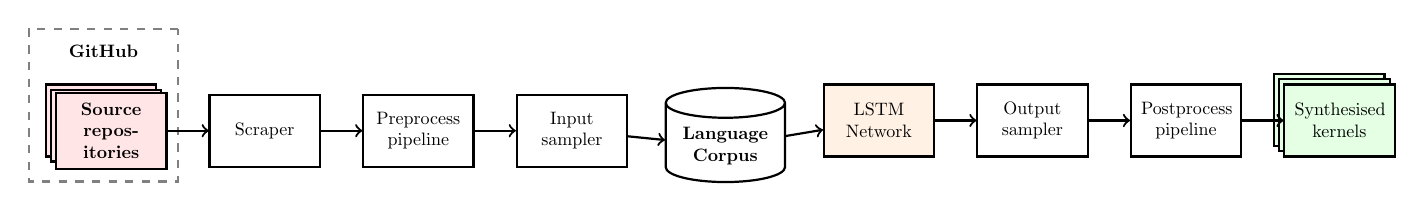
\begin{tikzpicture}[%
  auto,
  thick,
  scale=1,
  every node/.style={scale=0.65},
  node distance = 3cm,
  % Database shape:
  database/.style={%
    draw,
    cylinder,
    cylinder uses custom fill,
    shape border rotate=90,
    aspect=0.25
  }
  ]

  % Nodes:
  \node (t-start3) [block, fill=red!10, xshift=-.2cm, yshift=.2cm] {};
  \node (t-start2) [block, fill=red!10, xshift=-.1cm, yshift=.1cm] {};
  \node (t-start) [block, fill=red!10] {\textbf{Source repositories}};

  \node (t-scraper) [block, right of=t-start] {Scraper};
  \node (t-preprocess) [block, right of=t-scraper] {Preprocess pipeline};
  \node (t-input-sampler) [block, right of=t-preprocess] {Input sampler};
  \node (t-corpus) [database, right of=t-input-sampler, yshift=-.3cm] {\textbf{\begin{tabular}{c}Language\\Corpus\end{tabular}}};
  \node (t-network) [block, right of=t-corpus, fill=orange!10, yshift=.5cm] {LSTM Network};
  \node (t-output-sampler) [block, right of=t-network] {Output sampler};
  \node (t-postprocess) [block, right of=t-output-sampler] {Postprocess pipeline};
  \node (t-end3) [block, fill=green!10, right of=t-postprocess, xshift=-.2cm, yshift=.2cm] {};
  \node (t-end2) [block, fill=green!10, right of=t-postprocess, xshift=-.1cm, yshift=.1cm] {};
  \node (t-end) [block, fill=green!10, right of=t-postprocess] {Synthesised kernels};

  \node (github) [draw, dashed, color=gray, yshift=.5cm, xshift=-.15cm, inner ysep=1cm, inner xsep=.75cm, label={[yshift=-.7cm]\textbf{GitHub}}, fit=(t-start)] {};

  % Connectors:
  \draw[->] (t-start) -- (t-scraper);
  \draw[->] (t-scraper) -- (t-preprocess);
  \draw[->] (t-preprocess) -- (t-input-sampler);
  \draw[->] (t-input-sampler) -- (t-corpus);
  \draw[->] (t-corpus) -- (t-network);
  \draw[->] (t-network) -- (t-output-sampler);
  \draw[->] (t-output-sampler) -- (t-postprocess);
  \draw[->] (t-postprocess) -- (t-end);
\end{tikzpicture}

  \caption{%
    The kernel synthesis pipeline.%
  }
\label{fig:structure}
\end{figure*}


\section{Assembling Representative Benchmarks}\label{sec:}

We collect a large code corpus from
GitHub~\footnote{\url{https://github.com/}}. This took 2 days on a
single machine.

Alternative source of data: \emph{GHTorrent}~\cite{Gousios2014a}.

Rejection sampling to remove noise from dataset. Check that compiles.

Minimising non-functional variance using clang libraries and tools:
\begin{itemize}
\item Pre-process source to remove macros and conditional
  compilation.
\item Lossless vocabulary size reduction with AST rewriting of
  identifiers.
\item Automatically enforcing code style with formatting tools.
\end{itemize}

Proprocessing pipeline: Implemented on
LLVM\footnote{\url{http://llvm.org/}},
clang\footnote{\url{http://clang.llvm.org/}}, and
libclc\footnote{\url{http://libclc.llvm.org/}}.

 Compile to LLVM bytecode using libclc. Include
shim header which adds inferred values for common typedefs
(e.g. FLOAT_T to float), and best guesses for common constants
(e.g. WGSIZE).


\section{Learning the Implementation Space}\label{sec:ml}

Long Short-Term Memory~\cite{Hochreiter1997}. No features.

TODO: Plot distribution of representativeness from benchmark suites to
GitHub language model.


\section{Sampling Implementation Space}\label{sec:}

Given a function prototype.

Sample kernels with balanced brackets.

Rejection sampler.

Undefined behaviour.

Driver program (and dataset).

\lstset{language=[OpenCL]C}
\begin{lstlisting}[%
  frame=single,%
  caption=Parboil SGEMM benchmark.
]
__kernel void mysgemmNT( __global const float *A, int lda, __global const float *B, int ldb, __global float* C, int ldc, int k, float alpha, float beta )
{
    float c = 0.0f;
    int m = get_global_id(0);
    int n = get_global_id(1);

    for (int i = 0; i < k; ++i) {
	float a = A[m + i * lda];
	float b = B[n + i * ldb];
	c += a * b;
    }
    C[m+n*ldc] = C[m+n*ldc] * beta + alpha * c;
}
\end{lstlisting}


\lstset{language=[OpenCL]C}
\begin{lstlisting}[%
  frame=single,%
  caption=Transformed SGEMM implementation from preprocessing pipeline.
]
__kernel void A(__global const float *a, int b, __global const float *c, int d,
                __global float *e, int f, int g, float h, float i) {
  float j = 0.0f;
  int k = get_global_id(0);
  int l = get_global_id(1);

  for (int m = 0; m < g; ++m) {
    float n = a[k + m * b];
    float o = c[l + m * d];
    j += n * o;
  }
  e[k + l * f] = e[k + l * f] * i + h * j;
}
\end{lstlisting}


\lstset{language=[OpenCL]C}
\begin{lstlisting}[%
  frame=single,%
  caption=Example kernel synthesised from SGEMM function prototype.
]
TODO
\end{lstlisting}


\section{Experimental Methodology}\label{sec:evaluation}


\subsection{Experimental Setup}\label{subsec:}

\paragraph{Platforms} 2x GPUs, 1x CPU. Table~\ref{tab:platforms}


\begin{table}% tab:platforms
\scriptsize
\centering
\begin{tabular}{l l l l}
  \toprule
  & \textbf{Intel CPU} & \textbf{NVIDIA GPU} & \textbf{AMD GPU} \\
  \midrule
  \textbf{Model} & Core i7-2600 & GTX TITAN & Radeon 7970 \\
  \textbf{Frequency} & 3.6 GHz & 980 MHz & 1000 MHz \\
  \textbf{\#. Cores} & 8 & 2688 & 2048 \\
  \textbf{Memory} & 8 GB & 6 GB & 3 GB \\
  \textbf{Throughput} & 100 GFLOPS & 4494 GFLOPS & 3789 GFLOPS \\
  \bottomrule
\end{tabular}
\caption{Experimental platforms.}
\label{tab:platforms}
\end{table}


\paragraph{Benchmarks}

\begin{table}% tab:benchmarks
\scriptsize
\centering
\begin{tabular}{l r R{2cm} R{2cm}}
  \toprule
  & \textbf{Version} & \textbf{\#. seed kernels} & \textbf{\#. generated kernels}\\
  \midrule
  \textbf{Parboil~\cite{Stratton2012}} & 0.2 & 7 & x \\
  \textbf{PolyBench~\cite{Grauer-Gray2012}} & 1.0 & 30 & x \\
  \textbf{Rodinia~\cite{Che2009}} & 3.1 & 50 & x \\
  \textbf{SHOC~\cite{Danalis2010}} & 1.1.5 & 53 & x \\
  \textbf{AMD SDK} & 3.0 & x & x \\
  \textbf{NVIDIA SDK} & 4.2 & 36 & x \\
  \textbf{Synthetic} & - & - & x \\
  \bottomrule
\end{tabular}
\caption{%
  Benchmarks used.
}
\label{tab:benchmarks}
\end{table}

Table~\ref{tab:benchmarks}. Limitation of system: can't use kernels
with struct arguments as seeds.

Notes: Parboil: opencl\_base implementation. Rewrote typedefs.

Ignored kernels with structs: %
parboil-bfs, %
parboil-mri-q, %
rodinia-b-tree, %
rodinia-dwt2d, %
rodinia-heartwall, %
rodinia-lavamd, %
rodinia nearest neighour.


\paragraph{Datasets}

From Parboil.


\subsection{Methodology}

Followed the methodology of~\cite{Grewe2013}.

Statistical soundness.

Leave-one-out cross validation.


\section{Experimental Results}\label{sec:evaluation}


\subsection{Generated Compute Kernels}\label{subsec:}

What's the ratio of ``good'' code? How long did it take to sample?


\subsection{Qualitatively Evaluating Generated Code}\label{subsec:}

Human or
Robot~\footnote{\url{http://humanorrobot.uk/game?g=opencl&m=nitt}}. Related
works which have used Non-Interactive Turing
Tests~\cite{Gao2015a,Zhang2016}.


\subsection{Predicting Execution Device}\label{subsec:}

Classification accuracy.


\subsection{Comparison with State-of-the-Art}\label{subsec:}

Compare prediction performance with and without additional synthetic
benchmarks.


\section{Related Work}\label{sec:related-work}

Misc: Verifying GPU kernels~\cite{Betts2012}. Simulating OpenCL
kernels~\cite{Price2015}.

Machine Learning-based Performance Tuning:~\cite{Wen2015},
\cite{Magni2014}, \cite{Falch2015}. Domain specific:
Stencils~\cite{Garvey2015b}, \cite{Cummins2015a}. Input sensitive
autotuning~\cite{Ding2015}. Benchmark reduction~\cite{Castro2014}.


\subsection{Representative Benchmarking}

Designing worklaods~\cite{Eeckhout2002}.


\subsection{Program Generation}


\paragraph{Template-based} GENESIS~\cite{Chiu2015}.


\paragraph{Grammar-based} Fuzzers:
Csmith~\cite{Yang2012}, CLsmith~\cite{Pflanzer2016}.


\paragraph{Mutation-based} JVM fuzzing~\cite{Chena}.


\paragraph{Goal-oriented} Generating linear
transforms~\cite{Voronenko2009}, synthesising MapReduce
programs~\cite{Smith}, genearting data structure
implementations~\cite{Loncaric2016}.


\subsection{Mining Source Codes}

Neural Networks for representing programs~\cite{Bunel}.

Promises and perils of mining GitHub~\cite{Bird2009}.

Mining source code repositories at large
scale~\cite{Allamanis2013a,White2015a}. Machine learning for analysing
code~\cite{Allamanis2014a,Raychev}. Aiding software
engineering~\cite{Allamanis2014,Bird2015}.

Previous studies have involved data mining of GitHub for analysis of
software engineering
practises~\cite{Wu2014,Guzman2014,Baishakhi2014a,Vasilescu2015}.


\subsection{Deep Learning}

This is the first application of deep learning for synthesising
programs.

Deep Learning has been successful for synthesising graphics
textures~\cite{Gatys2015a}, image captions~\cite{Vinyals}, colors for
black and white photographs~\cite{Zhang2016}, and artistic
style~\cite{Gatys2015}.

DeepAPI learns API usage from annotated snippets from
GitHub~\cite{Zhang2015a}.


\section{Conclusion}\label{sec:conclusion}

Future work: probabilistic grammar.


\acks

This work was supported by the UK Engineering and Physical Sciences
Research Council under grants EP/L01503X/1 (CDT in Pervasive
Parallelism),\\* EP/H044752/1 (ALEA), and\\* EP/M015793/1 (DIVIDEND).


\label{bibliography}
\printbibliography


\end{document}
